\chapter{Healthy Habits}\label{ch:g1:healthy-habits}

Why does everyone keep saying ``wash your hands'', ``brush your
teeth'', ``off to bed''? Not to spoil the fun. Your body is the
\omterm{def:g1:living-or-not:living}{living thing} you will keep the longest --- your whole life --- and
a few small habits, done every day, keep it strong. Here is what
they are, and why they work.

\section{Keeping clean}

\begin{definition}[Germs]\label{def:g1:healthy-habits:germs}
\emph{Germs}\index{germ} are \omterm{def:g1:living-or-not:living}{living things} far too small to see,
which are everywhere --- on hands, on door handles, in dirt. Most
are harmless, but some can make us ill when they get inside the
body. Because they are invisible, hands that look clean can still
carry them.
\end{definition}

\begin{definition}[Hygiene]\label{def:g1:healthy-habits:hygiene}
\emph{Hygiene}\index{hygiene} means the habits that keep the body
clean and keep \omterm{def:g1:healthy-habits:germs}{germs} out: washing hands, washing the body, brushing
teeth, keeping food clean.
\end{definition}

\begin{method}[Washing hands well]\label{met:g1:healthy-habits:hands}
\begin{enumerate}
  \item Wet the hands and take soap;
  \item rub everywhere --- palms, backs, between the fingers,
        around the thumbs --- while you slowly count to $20$ or
        sing a short song;
  \item rinse under running water;
  \item dry with a clean towel.
\end{enumerate}
Wash before eating, after the toilet, and after playing outside or
touching \omterm{def:g1:animals-around-us:animal}{animals}.
\end{method}

\begin{omfigure}
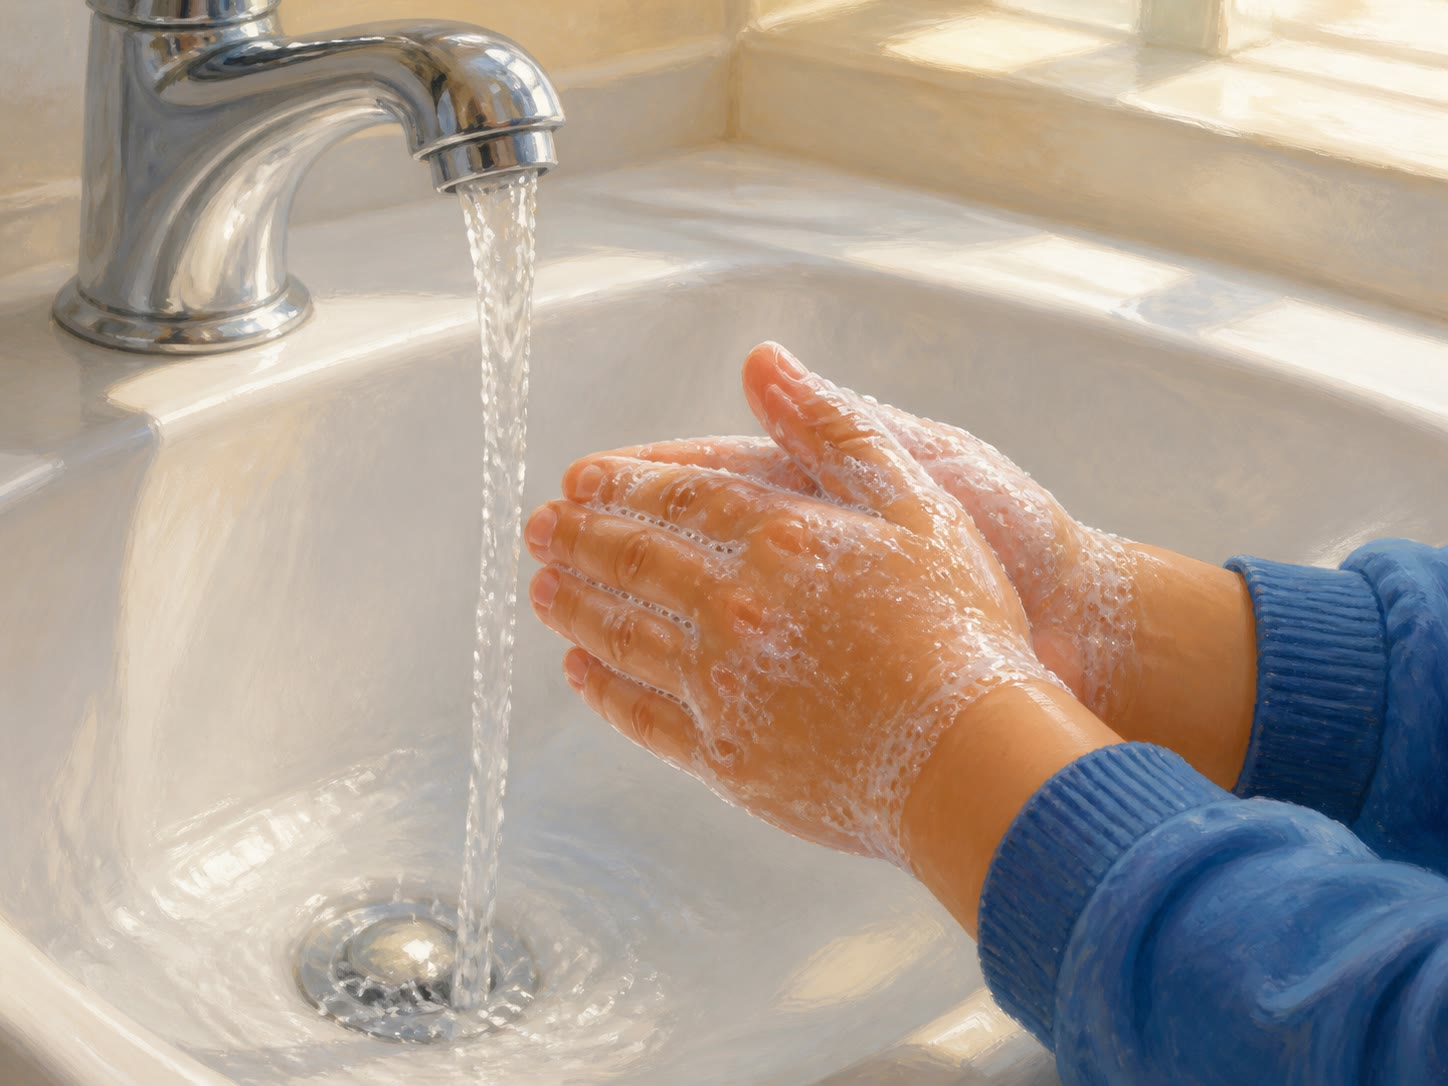
\includegraphics[width=0.58\linewidth]{images/book1/ai/g1-habits-handwashing.jpg}

{\small Soap, rubbing, running water: the \omterm{def:g1:healthy-habits:germs}{germs}' least favorite
song lasts a slow count of twenty.}
\end{omfigure}

\begin{example}[The glitter experiment]\label{ex:g1:healthy-habits:glitter}
Rub a pinch of glitter on your palms, then shake hands with a
friend, open a door, pick up a pencil: glitter everywhere. \omterm{def:g1:healthy-habits:germs}{Germs}
travel exactly like that, only invisibly. Now wash with soap,
counting to $20$ --- the glitter goes, and so do the \omterm{def:g1:healthy-habits:germs}{germs}.
\end{example}

\section{Teeth to keep}

\begin{proposition}[Why teeth must be brushed]\label{prop:g1:healthy-habits:teeth}
After eating, bits of food stay on the teeth. \omterm{def:g1:healthy-habits:germs}{Germs} in the mouth
feed on these leftovers --- especially the sugary ones --- and
slowly make holes in the teeth, which hurt. Brushing sweeps the
leftovers away before the \omterm{def:g1:healthy-habits:germs}{germs} can feast.
\end{proposition}
\admitted

\begin{method}[Brushing my teeth]\label{met:g1:healthy-habits:brush}
\begin{enumerate}
  \item Brush after breakfast and before bed --- every day;
  \item brush every side of every tooth: the front, the back, and
        the top where you chew;
  \item take your time --- about as long as a song;
  \item change to a new toothbrush when the bristles splay out.
\end{enumerate}
\end{method}

\begin{remark}[Baby teeth matter too]\label{rem:g1:healthy-habits:babyteeth}
``These teeth will fall out anyway --- why brush them?'' Because
they must chew for you for years yet, because holes in them hurt
just as much, and because the grown-up teeth are already waiting
underneath and deserve a clean, healthy mouth to arrive in.
\end{remark}

\section{Eating, moving, sleeping}

\begin{proposition}[The three daily needs]\label{prop:g1:healthy-habits:needs}
A growing body needs, every day:
\begin{enumerate}
  \item \emph{varied food}\index{varied food} --- a bit of
        everything: vegetables and fruit, bread and cereals, milk
        and cheese, meat or fish or eggs, and water to drink;
        sweets only now and then;
  \item \emph{movement}\index{movement} --- running, climbing,
        cycling, playing outside: moving makes muscles, bones and
        heart stronger;
  \item \emph{sleep}\index{sleep} --- at night the body rests,
        repairs itself and grows; a child needs a long night, far
        longer than a grown-up's.
\end{enumerate}
\end{proposition}
\admitted

\begin{omfigure}
\begin{tikzpicture}
  \draw[thick, omMeth, fill=omMeth!7, rounded corners=6pt]
    (0,0) rectangle (3.6,2.3);
  \draw[thick, omProp, fill=omProp!7, rounded corners=6pt]
    (4.0,0) rectangle (7.6,2.3);
  \draw[thick, omDef, fill=omDef!7, rounded corners=6pt]
    (8.0,0) rectangle (11.6,2.3);
  \node[font=\small\bfseries, omMeth] at (1.8,1.95) {eat varied};
  \node[font=\small\bfseries, omProp] at (5.8,1.95) {move};
  \node[font=\small\bfseries, omDef] at (9.8,1.95) {sleep};
  \node[font=\small, align=center, text width=3.3cm] at (1.8,0.9)
    {a bit of\\ everything,\\ water to drink};
  \node[font=\small, align=center, text width=3.3cm] at (5.8,0.9)
    {play outside,\\ run, climb,\\ every day};
  \node[font=\small, align=center, text width=3.3cm] at (9.8,0.9)
    {a long night:\\ the body repairs\\ and grows};
\end{tikzpicture}

{\small The three daily needs of a growing body. None of the three
can replace another.}
\end{omfigure}

\begin{example}[A good day for the body]\label{ex:g1:healthy-habits:day}
Breakfast with fruit; hands washed before lunch; an afternoon of
running in the park; teeth brushed after supper; lights out early
with a story. Nothing extraordinary --- and that is the point:
health is made of ordinary days like this one.
\end{example}

\begin{remark}[Tired is a message]\label{rem:g1:healthy-habits:tired}
Yawning, stinging \omterm{def:g1:the-five-senses:sense}{eyes}, grumpiness for no reason: that is the body
saying ``I need \omterm{prop:g1:healthy-habits:needs}{sleep}''. Listening to it is a healthy habit too.
A well-slept morning brain learns better, plays better and laughs
more easily.
\end{remark}

\section{Exercises}

\begin{exercise}[$\star$]\label{exo:g1:healthy-habits:1}
What are \omterm{def:g1:healthy-habits:germs}{germs}? Why can hands that look clean still need washing?
\end{exercise}

\begin{exercise}[$\star$]\label{exo:g1:healthy-habits:2}
Give three moments of the day when hands must be washed.
\end{exercise}

\begin{exercise}[$\star$]\label{exo:g1:healthy-habits:3}
In \cref{met:g1:healthy-habits:hands}, how long should the rubbing
with soap last? Name two spots that are easy to forget.
\end{exercise}

\begin{exercise}[$\star$]\label{exo:g1:healthy-habits:4}
Why do teeth get holes when they are not brushed? Tell the story
with the \omterm{def:g1:healthy-habits:germs}{germs} and the leftovers.
\end{exercise}

\begin{exercise}[$\star$]\label{exo:g1:healthy-habits:5}
When should teeth be brushed, and how long should it take?
\end{exercise}

\begin{exercise}[$\star$]\label{exo:g1:healthy-habits:6}
Name the three daily needs of \cref{prop:g1:healthy-habits:needs},
and one example of each from your own day.
\end{exercise}

\begin{exercise}[$\star$]\label{exo:g1:healthy-habits:7}
What does the body do during \omterm{prop:g1:healthy-habits:needs}{sleep}? Who needs the longer night, a
child or a grown-up?
\end{exercise}

\begin{exercise}[$\star$]\label{exo:g1:healthy-habits:8}
Give two signs that a body is asking for \omterm{prop:g1:healthy-habits:needs}{sleep}.
\end{exercise}

\begin{exercise}[$\star\star$]\label{exo:g1:healthy-habits:9}
Sam says: ``My baby teeth will fall out anyway, so brushing them
is useless.'' Answer him with
\cref{rem:g1:healthy-habits:babyteeth} --- two reasons at least.
\end{exercise}

\begin{exercise}[$\star\star$]\label{exo:g1:healthy-habits:10}
In the glitter experiment of \cref{ex:g1:healthy-habits:glitter},
what does the glitter stand for? What does the experiment show
about shaking hands --- and about soap?
\end{exercise}
